\documentclass{standalone}
\usepackage{tikz}
\usetikzlibrary{patterns, positioning}


\begin{document}
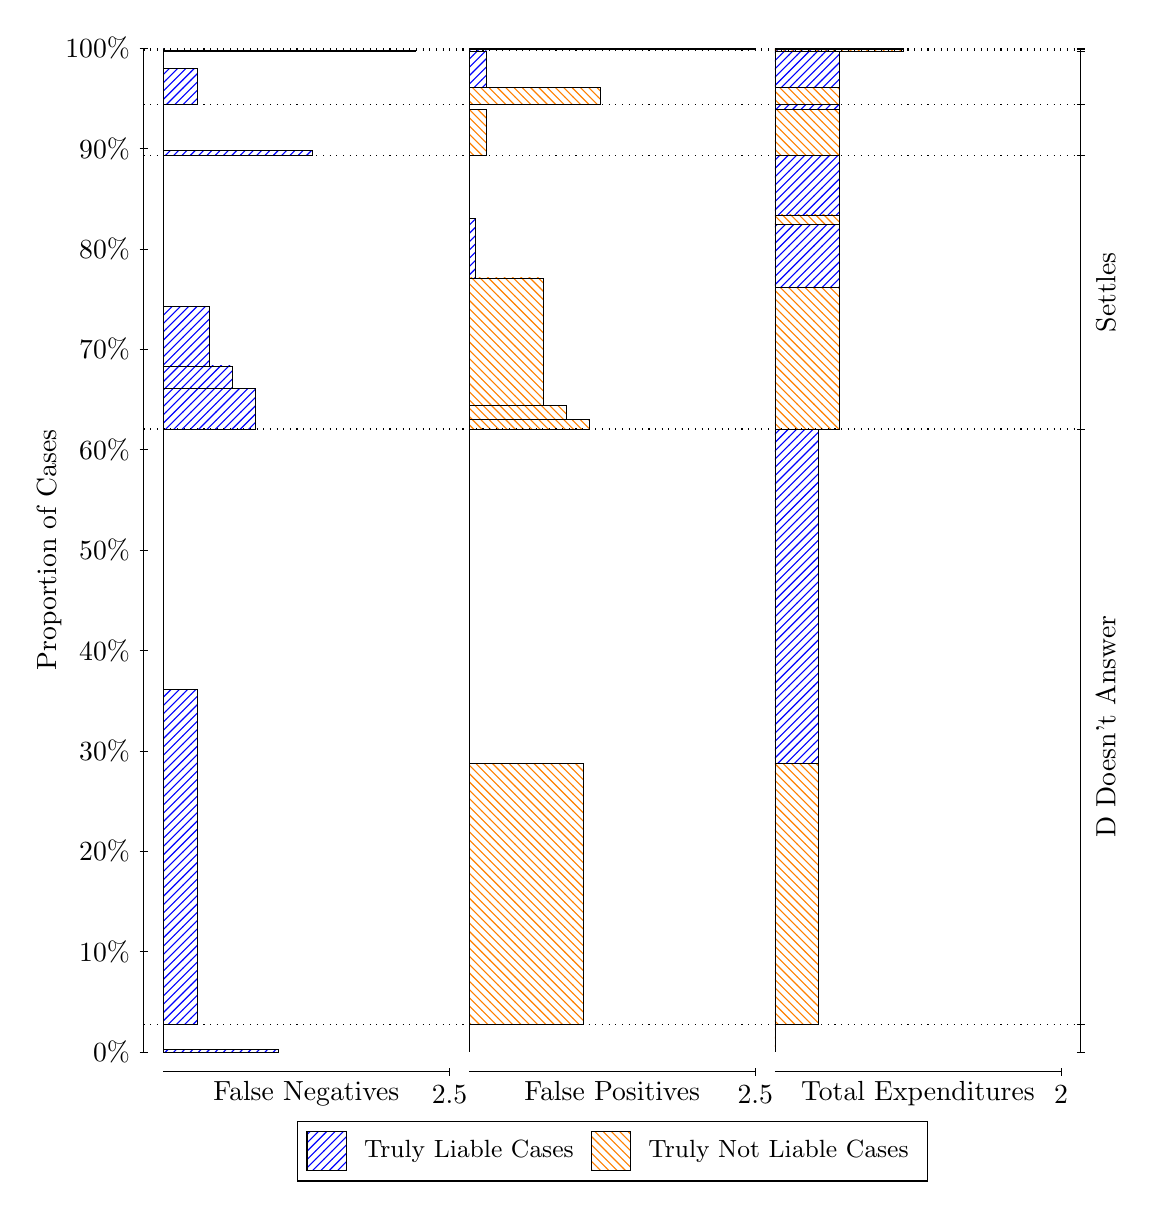
\begin{tikzpicture}
\draw[black, very thin] (1.5,1.75) -- (1.5,14.5);
\node[rotate=90, text=black, anchor=center] at (0.3, 8.125) {Proportion of Cases};
\draw[black, very thin] (1.45,1.75) -- (1.55,1.75);
\node[text=black, anchor=east] at (1.45, 1.75) {0\%};
\draw[black, very thin] (1.45,3.025) -- (1.55,3.025);
\node[text=black, anchor=east] at (1.45, 3.025) {10\%};
\draw[black, very thin] (1.45,4.3) -- (1.55,4.3);
\node[text=black, anchor=east] at (1.45, 4.3) {20\%};
\draw[black, very thin] (1.45,5.575) -- (1.55,5.575);
\node[text=black, anchor=east] at (1.45, 5.575) {30\%};
\draw[black, very thin] (1.45,6.85) -- (1.55,6.85);
\node[text=black, anchor=east] at (1.45, 6.85) {40\%};
\draw[black, very thin] (1.45,8.125) -- (1.55,8.125);
\node[text=black, anchor=east] at (1.45, 8.125) {50\%};
\draw[black, very thin] (1.45,9.4) -- (1.55,9.4);
\node[text=black, anchor=east] at (1.45, 9.4) {60\%};
\draw[black, very thin] (1.45,10.675) -- (1.55,10.675);
\node[text=black, anchor=east] at (1.45, 10.675) {70\%};
\draw[black, very thin] (1.45,11.95) -- (1.55,11.95);
\node[text=black, anchor=east] at (1.45, 11.95) {80\%};
\draw[black, very thin] (1.45,13.225) -- (1.55,13.225);
\node[text=black, anchor=east] at (1.45, 13.225) {90\%};
\draw[black, very thin] (1.45,14.5) -- (1.55,14.5);
\node[text=black, anchor=east] at (1.45, 14.5) {100\%};

\draw[black, very thin] (13.4,1.75) -- (13.4,14.5);
\draw[black, very thin] (13.35,1.75) -- (13.45,1.75);
\node[anchor=west] at (13.35, 1.75) {};
\draw[black, very thin] (13.35,2.1029) -- (13.45,2.1029);
\node[anchor=west] at (13.35, 2.1029) {};
\draw[black, very thin] (13.35,9.6615) -- (13.45,9.6615);
\node[anchor=west] at (13.35, 9.6615) {};
\draw[black, very thin] (13.35,13.137) -- (13.45,13.137);
\node[anchor=west] at (13.35, 13.137) {};
\draw[black, very thin] (13.35,13.786) -- (13.45,13.786);
\node[anchor=west] at (13.35, 13.786) {};
\draw[black, very thin] (13.35,14.463) -- (13.45,14.463);
\node[anchor=west] at (13.35, 14.463) {};
\draw[black, very thin] (13.35,14.487) -- (13.45,14.487);
\node[anchor=west] at (13.35, 14.487) {};
\draw[black, very thin] (13.35,14.5) -- (13.45,14.5);
\node[anchor=west] at (13.35, 14.5) {};

\draw[black, very thin, pattern color=blue, pattern=north east lines] (1.75,1.75) rectangle (3.2033,1.7871);
\draw[black, very thin, pattern color=orange, pattern=north west lines] (1.75,1.7871) rectangle (1.75,2.1029);
\draw[black, very thin, pattern color=blue, pattern=north east lines] (1.75,2.1029) rectangle (2.186,6.3505);
\draw[black, very thin, pattern color=orange, pattern=north west lines] (1.75,6.3505) rectangle (1.75,9.6615);
\draw[black, very thin, pattern color=blue, pattern=north east lines] (1.75,9.6615) rectangle (2.9127,10.18);
\draw[black, very thin, pattern color=blue, pattern=north east lines] (1.75,10.18) rectangle (2.622,10.462);
\draw[black, very thin, pattern color=blue, pattern=north east lines] (1.75,10.462) rectangle (2.3313,11.217);
\draw[black, very thin, pattern color=orange, pattern=north west lines] (1.75,11.217) rectangle (1.75,13.137);
\draw[black, very thin, pattern color=blue, pattern=north east lines] (1.75,13.137) rectangle (3.6393,13.201);
\draw[black, very thin, pattern color=orange, pattern=north west lines] (1.75,13.201) rectangle (1.75,13.786);
\draw[black, very thin, pattern color=blue, pattern=north east lines] (1.75,13.786) rectangle (2.186,14.245);
\draw[black, very thin, pattern color=orange, pattern=north west lines] (1.75,14.245) rectangle (1.75,14.463);
\draw[black, very thin, pattern color=blue, pattern=north east lines] (1.75,14.463) rectangle (4.9473,14.469);
\draw[black, very thin, pattern color=orange, pattern=north west lines] (1.75,14.469) rectangle (1.75,14.487);
\draw[black, very thin, pattern color=orange, pattern=north west lines] (1.75,14.487) rectangle (1.75,14.494);
\draw[black, very thin, pattern color=blue, pattern=north east lines] (1.75,14.494) rectangle (1.75,14.5);
\draw[black, very thin, pattern color=orange, pattern=north west lines] (5.6333,1.75) rectangle (5.6333,2.0658);
\draw[black, very thin, pattern color=blue, pattern=north east lines] (5.6333,2.0658) rectangle (5.6333,2.1029);
\draw[black, very thin, pattern color=orange, pattern=north west lines] (5.6333,2.1029) rectangle (7.0867,5.414);
\draw[black, very thin, pattern color=blue, pattern=north east lines] (5.6333,5.414) rectangle (5.6333,9.6615);
\draw[black, very thin, pattern color=orange, pattern=north west lines] (5.6333,9.6615) rectangle (7.1593,9.7809);
\draw[black, very thin, pattern color=orange, pattern=north west lines] (5.6333,9.7809) rectangle (6.8687,9.9644);
\draw[black, very thin, pattern color=orange, pattern=north west lines] (5.6333,9.9644) rectangle (6.578,11.582);
\draw[black, very thin, pattern color=blue, pattern=north east lines] (5.6333,11.582) rectangle (5.706,12.336);
\draw[black, very thin, pattern color=blue, pattern=north east lines] (5.6333,12.336) rectangle (5.6333,13.137);
\draw[black, very thin, pattern color=orange, pattern=north west lines] (5.6333,13.137) rectangle (5.8513,13.722);
\draw[black, very thin, pattern color=blue, pattern=north east lines] (5.6333,13.722) rectangle (5.6333,13.786);
\draw[black, very thin, pattern color=orange, pattern=north west lines] (5.6333,13.786) rectangle (7.3047,14.005);
\draw[black, very thin, pattern color=blue, pattern=north east lines] (5.6333,14.005) rectangle (5.8513,14.463);
\draw[black, very thin, pattern color=orange, pattern=north west lines] (5.6333,14.463) rectangle (5.6333,14.481);
\draw[black, very thin, pattern color=blue, pattern=north east lines] (5.6333,14.481) rectangle (5.6333,14.487);
\draw[black, very thin, pattern color=orange, pattern=north west lines] (5.6333,14.487) rectangle (9.2667,14.494);
\draw[black, very thin, pattern color=blue, pattern=north east lines] (5.6333,14.494) rectangle (7.8133,14.5);
\draw[black, very thin, pattern color=orange, pattern=north west lines] (9.5167,1.75) rectangle (9.5167,2.0658);
\draw[black, very thin, pattern color=blue, pattern=north east lines] (9.5167,2.0658) rectangle (9.5167,2.1029);
\draw[black, very thin, pattern color=orange, pattern=north west lines] (9.5167,2.1029) rectangle (10.062,5.414);
\draw[black, very thin, pattern color=blue, pattern=north east lines] (9.5167,5.414) rectangle (10.062,9.6615);
\draw[black, very thin, pattern color=orange, pattern=north west lines] (9.5167,9.6615) rectangle (10.334,11.462);
\draw[black, very thin, pattern color=blue, pattern=north east lines] (9.5167,11.462) rectangle (10.334,12.263);
\draw[black, very thin, pattern color=orange, pattern=north west lines] (9.5167,12.263) rectangle (10.334,12.382);
\draw[black, very thin, pattern color=blue, pattern=north east lines] (9.5167,12.382) rectangle (10.334,13.137);
\draw[black, very thin, pattern color=orange, pattern=north west lines] (9.5167,13.137) rectangle (10.334,13.722);
\draw[black, very thin, pattern color=blue, pattern=north east lines] (9.5167,13.722) rectangle (10.334,13.786);
\draw[black, very thin, pattern color=orange, pattern=north west lines] (9.5167,13.786) rectangle (10.334,14.005);
\draw[black, very thin, pattern color=blue, pattern=north east lines] (9.5167,14.005) rectangle (10.334,14.463);
\draw[black, very thin, pattern color=orange, pattern=north west lines] (9.5167,14.463) rectangle (11.152,14.481);
\draw[black, very thin, pattern color=blue, pattern=north east lines] (9.5167,14.481) rectangle (11.152,14.487);
\draw[black, very thin, pattern color=orange, pattern=north west lines] (9.5167,14.487) rectangle (11.152,14.494);
\draw[black, very thin, pattern color=blue, pattern=north east lines] (9.5167,14.494) rectangle (11.152,14.5);
\draw[black, dotted] (1.5,2.1029) -- (13.4,2.1029);
\draw[black, dotted] (1.5,9.6615) -- (13.4,9.6615);
\draw[black, dotted] (1.5,13.137) -- (13.4,13.137);
\draw[black, dotted] (1.5,13.786) -- (13.4,13.786);
\draw[black, dotted] (1.5,14.463) -- (13.4,14.463);
\draw[black, dotted] (1.5,14.487) -- (13.4,14.487);
\draw[black, very thin] (1.75,1.5) -- (5.3833,1.5);
\node[text=black, anchor=north] at (3.5667, 1.5) {False Negatives};
\draw[black, very thin] (5.3833,1.45) -- (5.3833,1.55);
\node[text=black, anchor=north] at (5.3833, 1.45) {2.5};

\draw[black, very thin] (5.6333,1.5) -- (9.2667,1.5);
\node[text=black, anchor=north] at (7.45, 1.5) {False Positives};
\draw[black, very thin] (9.2667,1.45) -- (9.2667,1.55);
\node[text=black, anchor=north] at (9.2667, 1.45) {2.5};

\draw[black, very thin] (9.5167,1.5) -- (13.15,1.5);
\node[text=black, anchor=north] at (11.333, 1.5) {Total Expenditures};
\draw[black, very thin] (13.15,1.45) -- (13.15,1.55);
\node[text=black, anchor=north] at (13.15, 1.45) {2};


\node[text=black, centered, rotate=90] at (13.72, 5.8822) {D Doesn't Answer};
\node[text=black, centered, rotate=90] at (13.72, 11.399) {Settles};





\draw (7.449999999999999,1.5) node[draw=none] (baseCoordinate) {};
\begin{scope}[align=center]
        \matrix[scale=0.5, draw=black, below=0.5cm of baseCoordinate, nodes={draw}, column sep=0.1cm]{
            \node[rectangle, draw, minimum width=0.5cm, minimum height=0.5cm, pattern color=blue, pattern=north east lines] {}; &
            \node[draw=none, font=\small, text=black] (B) {Truly Liable Cases}; &
            \node[rectangle, draw, minimum width=0.5cm, minimum height=0.5cm, pattern color=orange, pattern=north west lines] {}; &
            \node[draw=none, font=\small, text=black] (B) {Truly Not Liable Cases}; \\
            };
\end{scope}

\end{tikzpicture}
\end{document}